\documentclass{article}

\title{Physics 313-Fall 2023 9}
\author{Grant Saggars}
\date{Due 5:00 pm Nov. 8, 2023}

\usepackage{amsmath}
\usepackage{import}
\usepackage{pdfpages}
\usepackage{transparent}
\usepackage{xcolor}
\usepackage{framed}
\usepackage{enumerate}
\usepackage{geometry}
\usepackage{cancel}
\usepackage{silence}
% \WarningsOff*
% \ErrorsOff*
\usepackage{multicol}
\usepackage{lipsum}  
\usepackage{caption}
\usepackage{float}
% \usepackage{fontspec}
\usepackage{bbold}
\usepackage{pgfplots}
\pgfplotsset{compat=1.18}

\definecolor{shadecolor}{RGB}{235,235,235}

\geometry{top=1in, bottom=1in, left=1in, right=1in}
\newenvironment{callout}[1] {\begin{shaded*} \textbf{#1}} {\end{shaded*}}

%%%%%%%%%%%%%%%%%%%%%%%%
% DOCUMENT BEGINS HERE %
%%%%%%%%%%%%%%%%%%%%%%%%

\begin{document}

\maketitle

\begin{enumerate}
    \item (3 pts) (Heisenberg Uncertainty) The speed of an electron is measured to within an uncertainty of $2.0 \times 10^{4}$ m/s. What is the size of the smallest region in which it can be confined?

        \begin{callout}{Solution:}

            Using let $v_e=\alpha \pm 2.0\times10^4$; using $\Delta x \Delta p \geq \frac{\hbar}{2}$:
            \begin{align*}
                \Delta x (2.0 \times 10^{4}) &\geq \frac{\hbar}{2} \\
                \implies \Delta x &\geq \frac{\hbar}{4 \times 10^{4}}
            \end{align*}

            This implies that the smallest region in which the electron can be confined is $\frac{\hbar}{4 \times 10^{4}}$ m.
        \end{callout}

    \item (3 pts) Doors are about 1 m wide, and human beings are very roughly 160 lbs. How slow would a person have to be moving through a doorway in order for that person to diffract?

        \begin{callout}{Solution:}

            The De Broglie wavelength of a human being is $\frac{h}{p}$, and destructive interference occurs when $a \sin(\theta) = m \lambda$. Therefore, for a human to diffract, both sides of the equation would need to be proportional.
            \begin{align*}
                a &= \lambda \to a \sim \frac{h}{mv} \\
                \implies v &\sim \frac{h}{ma} \\
                &\sim 9.135 \times 10^{-36} \textrm{m/s}
            \end{align*}
        \end{callout}

    \newpage
    \item (4 pts) Consider two waves $\cos(2\pi x/\lambda_1)$ and $\cos(2\pi x/\lambda_2)$ where $\lambda_1 = 1$ m and $\lambda_2 = 1.1$ m. In your favorite plotting program, plot each wave separately and then plot the addition of the waves assuming equal amplitude. Do it over the range $-15$ m $< x < 15$ m. Do you see beats when you add them together?

    \begin{callout}{Plot:}

        The beats are clearly defined in the plot below:

    \center
    \resizebox{0.9\textwidth}{!}{%
        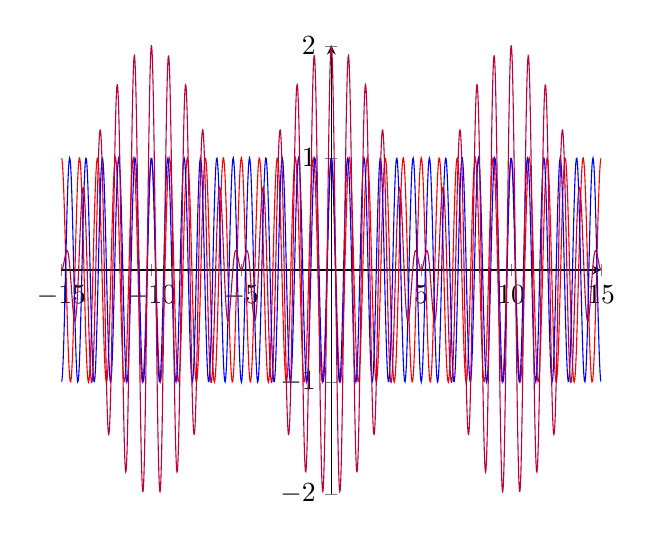
\begin{tikzpicture}
            \begin{axis}[
            xmin=-15, xmax=15,
            ymin=-2, ymax=2,
            axis lines=middle,]
            \addplot[domain=-15:15, samples=1000, red]{cos(deg(2 * pi * x))};
            \addplot[domain=-15:15, samples=1000, blue]{cos(deg(1.1 * 2 * pi * x))};
            \addplot[domain=-15:15, samples=2000, purple]{cos(deg(1.1 * 2 * pi * x)) + cos(deg(2 * pi * x))};
        \end{axis}
        \end{tikzpicture}
    }
    \end{callout}

\end{enumerate}

\end{document}
